%Validation PoC
\chapter{Proof of Concept Validation}
\label{pocvalid:chapter}
In diesem Kapitel wird folgende Frage beantwortet: \textit{''Ist eine praxistaugliche Software, die die Problemstellung des Auftrags erfüllt, möglich?''}.\\

Das Kapitel ist dabei in die Teile Validation des Prototyps V1 im Abschnitt \ref{pocvalid:v1} und die Validation des Prototyps V2 im Abschnitt \ref{pocvalid:v2} unterteilt.

%Testing Prototype V1
\section{Testing Prototyp V1}
\label{pocvalid:v1}
In diesem Abschnitt wurde der Prototyp V1 getestet, ob dieser die Anforderungen abdeckt.
\subsection{Infrastruktur}
Die Software wird lokal ausgeführt, und alle Services werden automatisch gestartet.

\subsection{Testfälle}
Die Testfälle werden mit dem Pattern P1 (für Prototyp V1) gekennzeichnet.


\begin{table}[H]
	\subsubsection{P1-T1: Software ausführen}
    \centering
	\begin{tabularx}{\textwidth}{| l | p{0.6\textwidth} |}
        \hline
        \textbf{ID/Bezeichnung} & P1-T01 - Software starten\\ \hline
        \textbf{Beschreibung} &  \\ \hline  
        \textbf{Testvoraussetzung} & Prototyp V1 aufgesetzt, lauffähig und alle benötigen Libraries installiert. \\ \hline      
        \textbf{Testschritte} & \begin{enumerate}
        	\item Software starten
        	\item Ausgabe auf Kommandozeile interpretieren
        \end{enumerate} \\ \hline    
        \textbf{Erwartetes Ergebnis} & Die Software startet und sendet dabei HTTP und HTTPS Request an verschiedene Ziele. Requests, die einen Malware Header beinhalten, werden dabei auf den Fake \gls{cc} HTTP/HTTPS Server umgeleitet. \\ \hline      
    \end{tabularx}
    \caption{Validation: Prototyp V1 Testfall 1}
\end{table}




\subsection{Testprotokoll}
\subsubsection{Protokoll Testfall P1-T1}
Software hat gestartet und angefangen, HTTP und HTTPS Requests zu machen, dabei werden einem alle offenen Sessions angezeigt.
Dabei sind vor allem die Responses vom Localhost interessant, der Fake \gls{cc} bekommt also umgeleitete Requests und antwortet auf diese, somit scheint der Layer 7 redirect zu funktionieren.

\begin{figure}[H]
	\centering
	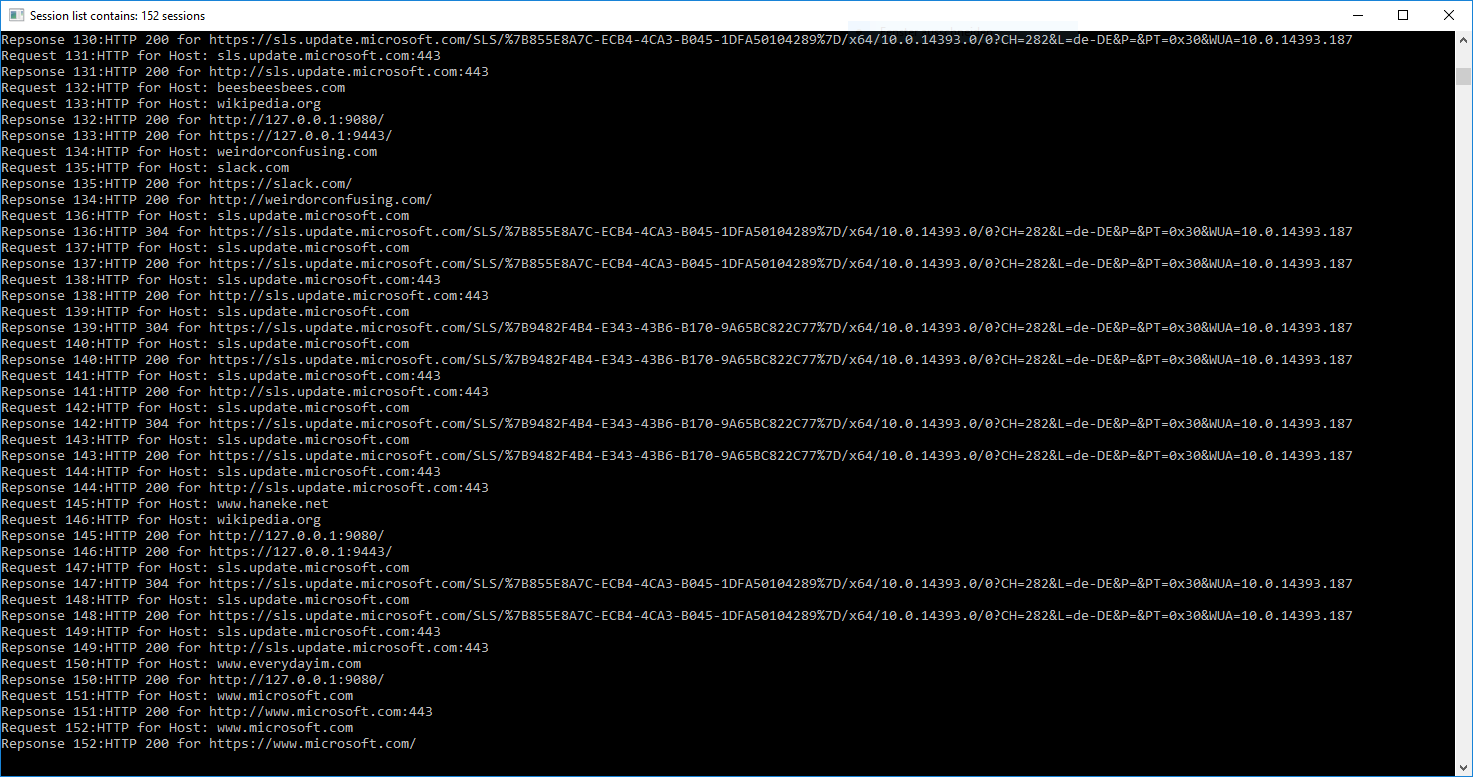
\includegraphics[width=\textwidth]{img/sessionlist.png}
	\caption{Validation: Session List von FiddlerCore}
	\label{fig:fiddler-core-session-list}
\end{figure}


\paragraph{HTTP Connect Host}
Da bei jeder HTTPS Verbindung ein HTTP Connect Request gesendet wird, welcher nur den Host beinhaltet, kann nicht anhand des Headers umgeleitet werden, die nachfolgenden Requests schon.
Somit müsste der Host bekannt sein, den man weiterleiten möchte, ohne diesen geht es nicht.

\begin{listing}[H]
\begin{fancycode}
CONNECT 127.0.0.1:8877 HTTP/1.1
Host: wikipedia.org
Proxy-Connection: Keep-Alive
\end{fancycode}
\caption{Validation: HTTP Connect Beispiel}
\label{lst:http-connect}
\end{listing}


\subsection{Zusammenfassung}
Layer 7 Redirect funktioniert zwar, aber der CONNECT Request kann so oder so nicht direkt abgefangen werden, es sei denn, man kennt den Host bevor man umleitet.
Durch diese Erkenntnis entschieden wir uns, einen weiteren Prototypen zu erstellen, der auf eine zeitversetzte Erkennung setzt.

%Testing Prototype V1

%Testing Prototype V2
\section{Testing Prototyp V2}
\label{pocvalid:v2}
In diesem Abschnitt wurde der Prototyp V2 getestet.
\subsection{Infrastruktur}
Der Prototyp V2 wurde auf der Testumgebung getestet, und um eine Malware nachzubilden, wurde eine einfache Client-Server Applikation geschrieben.
\subsection{Testfälle}
Die Testfälle werden mit dem Pattern P2 (für Prototyp V2) gekennzeichnet.


\begin{table}[H]
\subsubsection{P2-T1: Über Squid Proxy Browsen}
    \centering
	\begin{tabularx}{\textwidth}{| l | p{0.6\textwidth} |}
        \hline
        \textbf{ID/Bezeichnung} & P2-T01 - Über Squid Proxy Browsen\\ \hline
        \textbf{Beschreibung} &  \\ \hline  
        \textbf{Testvoraussetzung} & Prototyp V2 aufgesetzt und konfiguriert. Test Client im gleichen Netz wie Proxy. \\ \hline      
        \textbf{Testschritte} & \begin{enumerate}
        	\item CURL GET auf Example.com
        	\item CURL POST auf Example.com mit Body
        	\item CURL PUT auf Example.com mit Body
        	\item Auf Kibana überprüfen, ob Requests geloggt wurde
        \end{enumerate} \\ \hline    
        \textbf{Erwartetes Ergebnis} & Alle gemachten Requests mit CURL werden in Kibana angezeigt und somit durch den Prototyp V2 geloggt. \\ \hline      
    \end{tabularx}
    \caption{Validation: Prototyp V2 Testfall 1}
\end{table}



\begin{table}[H]
\subsubsection{P2-T2: Redirect provozieren}
    \centering
	\begin{tabularx}{\textwidth}{| l | p{0.6\textwidth} |}
        \hline
        \textbf{ID/Bezeichnung} & P2-T01 - Redirect provozieren\\ \hline
        \textbf{Beschreibung} &  \\ \hline  
        \textbf{Testvoraussetzung} & Prototyp V2 aufgesetzt und konfiguriert Test Client im gleichen Netz wie Proxy. Keine Iptable gesetzt, die bereits umleitet. \\ \hline      
        \textbf{Testschritte} & \begin{enumerate}
        	\item CURL POST mit Body, der einem Suchpattern entspricht
        	\item Auf Kibana prüfen,ob geloggt wurde
        	\item Nochmaliger CURL POST auf gleichen Destination Host
        	\item Rückmeldung nun vom Fake \gls{cc} Server
        \end{enumerate} \\ \hline    
        \textbf{Erwartetes Ergebnis} & Der Request triggert den Triggerfish und dieser setzt über den Mandarinfish eine Iptable, dadurch wird der nächste Request an den gleichen Host auf den Fake \gls{cc} umgeleitet.\\ \hline      
    \end{tabularx}
    \caption{Validation: Prototyp V2 Testfall 2}
\end{table}



\begin{table}[H]
\subsubsection{P2-T3: Pseudo Malware}
    \centering
	\begin{tabularx}{\textwidth}{| l | p{0.6\textwidth} |}
        \hline
        \textbf{ID/Bezeichnung} & P2-T01 - Pseudo Malware\\ \hline
        \textbf{Beschreibung} &  \\ \hline  
        \textbf{Testvoraussetzung} & Prototyp V2 aufgesetzt und konfiguriert Test Client im gleichen Netz, wie Proxy. Keine Iptable gesetzt, die bereits umleitet. ''Original \gls{cc}'' erreichbar. \\ \hline      
        \textbf{Testschritte} & \begin{enumerate}
        	\item Client starten und abwarten
        	\item Kibana prüfen, ob geloggt wird
        	\item Rückgaben auf Kommandozeile überprüfen
        \end{enumerate} \\ \hline    
        \textbf{Erwartetes Ergebnis} & Der Client sendet fortlaufend Requests, welche durch den ''Original \gls{cc}'' bestätigt werden, auf der Kommandozeile kann das nachvollzogen werden, sobald die Umschaltung auf den Fake \gls{cc} stattfand.\\ \hline      
    \end{tabularx}
    \caption{Validation: Prototyp V2 Testfall 3}
\end{table}


\subsection{Testprotokoll}
\subsubsection{P2-T1: Über Squid Proxy Browsen}
Es sollen nun 3 Requests über den Squid Proxy gemacht werden, und diese müssen vom Pufferfish Logger geloggt werden und in die Elasticsearch gespeichert werden.\\


\begin{listing}[H]
\textbf{GET}\\
\begin{fancycode}
curl http://example.com --proxy mandarin:3128
\end{fancycode}
\caption{Validation: CURL GET über Proxy}
\label{lst:curl-get-proxy}
\end{listing}


\begin{listing}[H]
\textbf{POST}\\
\begin{fancycode}
curl http://example.com -X POST -d "{"count":4000}" --proxy mandarin:3128
\end{fancycode}
\caption{Validation: CURL POST über Proxy}
\label{lst:curl-post-proxy}
\end{listing}

\begin{listing}[H]
\textbf{PUT}\\
\begin{fancycode}
curl http://example.com -X PUT -d "{"count":4000}" --proxy mandarin:3128
\end{fancycode}
\caption{Validation: CURL PUT über Proxy}
\label{lst:curl-put-proxy}
\end{listing}

Sobald alle Requests durchgeführt wurden, sollte dies nun im Kibana auftauchen und dank Elasticsearch durchsuchbar sein.


\begin{figure}[H]
	\centering
	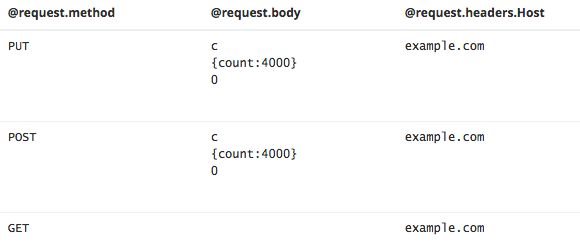
\includegraphics[width=0.75\textwidth]{img/requests-kibana}
	\caption{Validation: Requests in Kibana}
	\label{fig:kibana-request}
\end{figure}



\subsubsection{P2-T2: Redirect provozieren}
Der Triggerfish sucht nach dem Pattern ''100'', sobald 1 Request gemacht wird, der dieses Pattern beinhaltet, muss eine Iptable auf dem Mandarinfish existieren, welche den Destination Host auf den Fake \gls{cc} umleitet.

\begin{listing}[H]
\begin{fancycode}
curl http://example.com -X POST -d "{"count":100}" --proxy mandarin:3128
\end{fancycode}
\caption{Validation: Request mit POST 100}
\label{lst:request-post-100}
\end{listing}

Nach den Requests muss also nach kurzer Zeit eine Iptable auf dem Mandarin Host existieren, die alle Requests auf den Fake C\&C umleitet.

\begin{listing}[H]
\begin{fancycode}
Chain PREROUTING (policy ACCEPT)
target     prot opt source               destination         

Chain INPUT (policy ACCEPT)
target     prot opt source               destination         

Chain OUTPUT (policy ACCEPT)
target     prot opt source               destination         
DNAT       all  --  anywhere             [Destination IP]        to:[FakeCC IP]

Chain POSTROUTING (policy ACCEPT)
target     prot opt source               destination 
\end{fancycode}
\caption{Validation: Iptables List}
\label{lst:Iptables-list}
\end{listing}

Sobald nochmals ein neuer Request gemacht wird auf den gleichen Host, kommt der Response vom Fake \gls{cc}.

\begin{listing}[H]
\begin{fancycode}
curl http://example.com -X POST -d "{"count":100}" --proxy mandarin:3128
#Fake C&C Repsonse
Cannot POST /
\end{fancycode}
\caption{Validation: Erneuter Request an Example.com}
\label{lst:request-example-new}
\end{listing}

\subsubsection{P2-T3: Pseudo Malware}
Nun soll das ganze dynamisch getestet werden, dazu wurde eine Software programmiert, welche einen einfachen Counter hoch zählt. Sobald dieser 100 erreicht hat, muss ein Redirect gesetzt werden.

Der Fake \gls{cc} zählt dabei um 100 hoch, man sieht auf der Konsole, sobald die Umschaltung stattgefunden hat.

\begin{listing}[H]
\begin{jscode}
14 Second
send: 100
{"count":101}
16 Second
send: 102
{"count":103}
17 Second
send: 104
{"count":105}
18 Second
send: 106
{"count":107}
19 Second
send: 108
{"count":109}
20 Second
send: 110
{"count":210}
22 Second
send: 211
{"count":311}
\end{jscode}
\caption{Validation: Client Requests an den Server}
\label{lst:client-request-server}
\end{listing}
Die Umleitung benötigte knappe 6 Sekunden, danach wurde auf den Fake \gls{cc} Server umgeleitet.


\subsection{Zusammenfassung}
Der Redirect funktioniert, allerdings müsste die Reaktionszeit noch verbessert werden, da momentan noch nicht entschlüsselt werden muss.
Dies ist aber dank der Separierung der Systeme relativ gut möglich, so kann jeder Service in der Performance verbessert werden.

%Testing Prototype V2

\section{Schlussfolgerung}
Der Prototyp V1 hat nicht vollständig so funktioniert wie geplant, da eine Echtzeit Analyse nicht so einfach zu bewerkstelligen ist.
Der Prototyp V2 hat allerdings gute Erfolgsaussichten, alleine schon durch die Aufteilung in verschiedene eigene Systeme.




